\section{Introduction}
Before we dive into our work, we must introduce the key concepts that we had to understand in order to build our project.
\subsection{Neural Machine Translation}
Neural Machine Translation, or simply NMT, is an approach to translate sentences from one language into another one (e.g.: from english to italian) by using a single neural network whose architecture is based on the encoder-decoder paradigm.
\vspace{3mm}
\subsubsection{Seq2Seq model}\label{subsubsec:seq2seq_model}
In its easiest form the network is composed by two RNNs (LSTMs or GRUs), one for the encoder and one for the decoder, that are trained jointly, in an end-to-end fashion, for maximizing the translation performance; such model composed of two RNNs is called sequence-to-sequence, or seq2seq in short, and its way of working is extremely straight forward:
\begin{itemize}
    \item The encoder receives one sentence from the source language and produces an encoding from it, such encoding will provide the fist hidden state of the decoder;
    \item The decoder receives the encoding produced by the encoder and builds the sentence in the target language one word at time conditioned on the encoding.
\end{itemize}
\begin{figure}[H]%
    \centering
    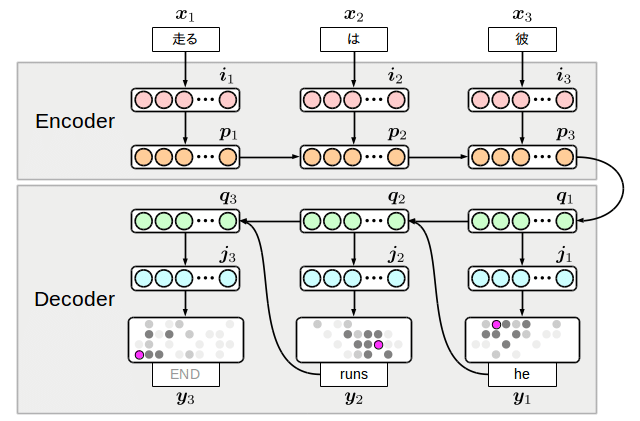
\includegraphics[width=0.74\linewidth]{images/seq2seq.png}
    \caption{Seq2seq model with no attention mechanism} %\cite{VanLandeghem_seq2seq}}
    \label{fig:seq2seq_model_no_attention}
\end{figure}

We said that the encoder generates the final sentence conditioned on what the encoder did, so the seq2seq model is a Conditional Language Model where the target sentence is built from predictions conditioned on the source sentence, so a seq2seq model, and more generally a NMT model, works as if it is calculating a probability distribution P(y|x) where y is the target sentence and x is the source one; more generally we can state the following formula:
\begin{large}
$$P(y|x)=P(y_{1}|x)P(y_{2}|y_{1},x)...P(y_{n}|y_{1..n-1},x)$$
\end{large}

NMT models are the the current state-of-art models in the machine translation field, but, as every model known, they have their pros and cons:
\begin{itemize}
    \item They beat all previous models by a large margin, providing more fluent and precise context-wise translations;
    \item They only use one single network whose parts (encoder and decoder) are trained together giving less headaches on optmizing every single sub-module;
    \item However their work is less interpretable from a human side and we can't specify any rules that would help our translations;
    \item For a simple seq2seq model if we need to translate long sentences we may lose the context and the weight of words far from the current encoding.
\end{itemize}
\subsubsection{Attention mechanism}
To counteract the last issue (losing context on long sentences) and to prevent bottleneck problems in the link beetween the encoder and decoder, the attention mechanism was introduced. At each decoding step our model focus only on one particular part of the source sentence. 
\vspace{3mm}

Figure \ref{fig:attention_mechanism} shows how the attention mechanism is integrated in a seq2seq model, however its use is not limited to this kind of architecture and many types of attention exist and we'll show some of them in section \ref{subsec:transformer_model}, where we will discuss about multi-head and self-attention.
\begin{figure}[H]%
    \centering
    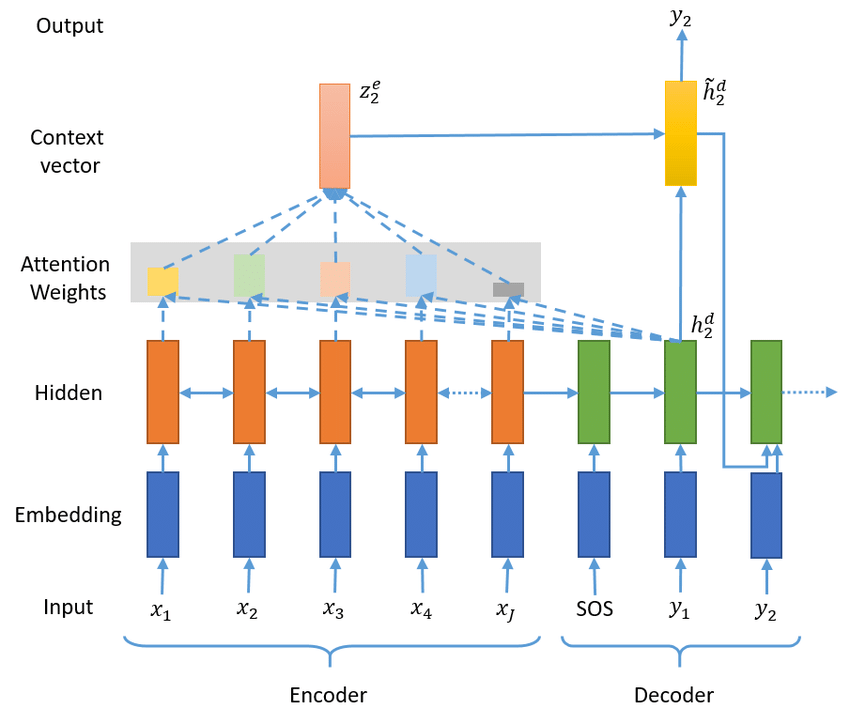
\includegraphics[width=0.68\linewidth]{images/attention_mechanism_2.png}
    \caption{Attention mechanism in a seq2seq model}
    \label{fig:attention_mechanism}
\end{figure}
The attention mechanism greatly improved the performance of NMT models not only solving the previous issues we mentioned but even solving the vanishing gradient problem that affects very deep networks and provides some interpretability to our model, something that we base NMT models lacked.
\vspace{3mm}

It's important to highlight the fact that the attention mechanism is not only useful in the context of machine translation since it's commonly used in other Natural Language Tasks and even in machine vision, this makes attention an highly versatile and vital mechanism.
\subsection{Transformer Model}\label{subsec:transformer_model}
In \ref{subsubsec:seq2seq_model} we've seen a very simple model composed by two RNNs, one for the encoder and one for the decoder, but a more powerful and complex architecture was introduced by Vaswani et al.\cite{vaswani2017attention} called transformer that disposes of any recurrent or convolutional layer and relies solely on attention. The transformer still follows the encoder-decoder paradigm, but both are now composed by multiple layers and sub-layers:
\begin{itemize}
    \item \textbf{Encoder}\\
    The encoder is composed of a stack of N identical layers and each layer has two sub-layers. The first is a multi-head self-attention mechanism, and the second is a position-wise fully connected feed-forward network. Each of the two sub-layers is followed by layer normalization. All sub-layers in the model, as well as the embedding layer, produce outputs of the same dimension.
    \item \textbf{Decoder}\\
    The decoder is also composed of a stack of N identical layers. The decoder inserts a third sub-layer, which performs multi-head attention over the output of the encoder stack. Similar to the encoder, each of the sub-layers is followed by layer normalization. We also modify the self-attention sub-layer in the decoder stack to prevent positions from attending to subsequent positions. This masking, combined with fact that the output embeddings are offset by one position, ensures that the predictions for position i can depend only on the known outputs at positions less than i.
\end{itemize}
\begin{figure}[H]%
    \centering
    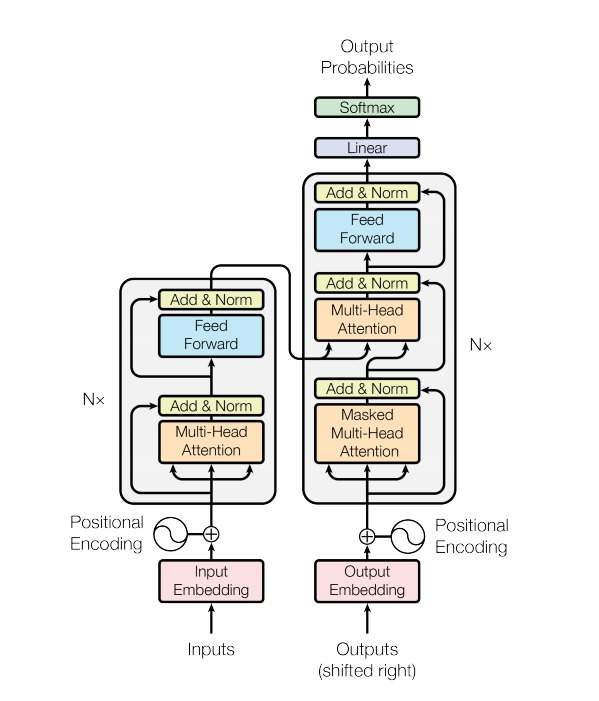
\includegraphics[width=0.68\linewidth]{images/transformer.png}
    \caption{Transformer model}
    \label{fig:transformer}
\end{figure}
\subsubsection{Self and multi-head attention}
The particular attention used by Vaswani et al.\cite{vaswani2017attention} is called "Scaled Dot-Product Attention" or self-attention (Figure \ref{fig:transformer_attention} on the right). The input consists of queries and keys of dimension $dk$, and values of dimension $dv$. We compute the dot products of the query with all keys, divide each by $\sqrt{dk}$, and apply a softmax function to obtain the weights on the values.
\begin{figure}[H]%
    \centering
    \subfloat[Multi-Head Attention]{{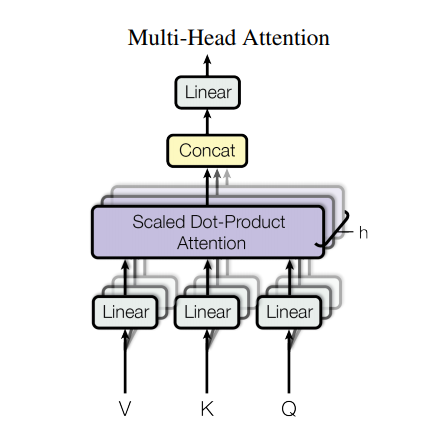
\includegraphics[width=0.50\linewidth]{images/multi_head_attention.png}}}%
    \subfloat[Self-Attention]{{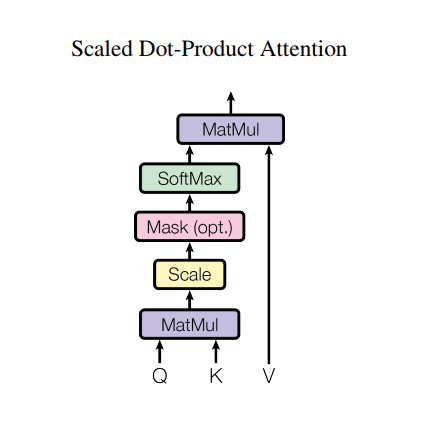
\includegraphics[width=0.50\linewidth]{images/self_attention.png}}}%
    \caption{On the left the multi-head attention is shown composed by multiple heads (self-attentions), on the right the single self-attention mechanism.}
    \label{fig:transformer_attention}%
\end{figure}
The attention function is computed on a set of queries simultaneously, packed together into a matrix Q. The keys and values are also packed together into matrices K and V . We compute the matrix of outputs as:
\begin{large}
$$Attention(Q, K, V ) = softmax(\frac{QK^T}{\sqrt{dk}})V$$
\end{large}

Instead of performing a single attention function with keys, values and queries whose dimension is based on the model dimension, it is beneficial to linearly project the queries, keys and values h times with different, learned linear projections to dk, dk and dv dimensions, respectively. On each of these projected versions of queries, keys and values we then perform the attention function in parallel, yielding $dv$-dimensional output values. These are concatenated and once again projected, resulting in the final values, as depicted in Figure \ref{fig:transformer_attention} on the left.
Multi-head attention allows the model to jointly attend to information from different representation subspaces at different positions.
\begin{large}
$$MultiHead(Q, K, V ) = Concat(head_{1}, ..., head_{h})W^O$$
\begin{center}where\end{center}
$$head_{i} = Attention(QW^Q_{i}, KW^K_{i}, VW^V_{i})$$
\end{large}

If we call h as the number of parallel attention layers, or heads, for each of these we use $dk=dv=dmodel/h$ as dimension. Due to the reduced dimension of each head, the total computational cost is similar to that of single-head attention with full dimensionality.
\subsection{BERT}
BERT (Biderectional Encoder Representations from Transformers) is a multi-layer bidirectional Transformer encoder introduced by Drevlin et al. \cite{devlin2018bert} and  based on the original transformer implementation described in Vaswani et al.\cite{vaswani2017attention}.
\begin{figure}[H]%
    \centering
    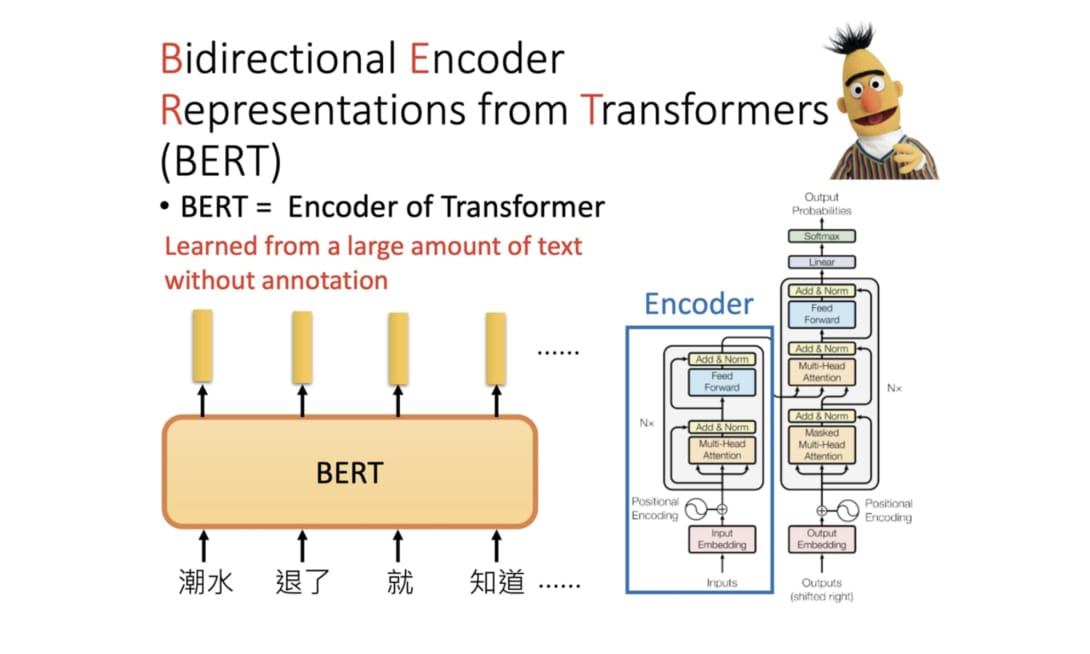
\includegraphics[width=1\linewidth]{images/BERT.png}
    \caption{BERT transformer}
    \label{fig:bert_transformer}
\end{figure}

BERT is conceptually simple and empirically powerful and that's why we used it in our project, even though its use is not aimed at NMT (it is aimed at masked language tasks) it still provides great performances for our work.
\vspace{3mm}

For our project we used a pre-trained versione of BERT from the Huggingface portal, from where also we used the tokenizer needed to let BERT work without any issue, we'll talk about this in chapter \ref{sec:project_task}.